\documentclass[conference]{IEEEtran}
\usepackage{graphicx, multicol, latexsym, amsmath, amssymb}
\usepackage{blindtext}
\usepackage{subfigure}
\usepackage{caption}
\usepackage{multirow}
\usepackage{booktabs}
\usepackage[justification=centering]{caption}
\usepackage{ragged2e}
\usepackage[table,xcdraw]{xcolor}
%\usepackage[tableposition=top]{caption}
%\usepackage{tabularx}
%\usepackage{capt-of}
%\usepackage{tabu}
%\usepackage{hyperref}
%\usepackage{booktabs}% for better rules in the table
%\usepackage{anysize} % Soporte para el comando \marginsize
%\usepackage{adjustbox}
\usepackage{float}
\usepackage{wrapfig}
\ifCLASSINFOpdf
\else
\fi
\hyphenation{op-tical net-works semi-conduc-tor}
%\pagenumbering{roman}
\pagestyle{plain}
\begin{document}

\title{End-To-End Framework for Keyword Spotting}
\author{\IEEEauthorblockN{Stefano Ivancich}
\IEEEauthorblockA{Department of\\Information Engineering\\
University of Padova, Italy\\
Email: stefano.ivancich@studenti.unipd.it}
\and
\IEEEauthorblockN{Luca Masiero}
\IEEEauthorblockA{Department of\\Information Engineering\\
University of Padova, Italy\\
Email: luca.masiero.8@studenti.unipd.it}}

\maketitle

\begin{abstract}
In this paper we present an end-to-end approach for the Keyword Spotting task: it consists of a sliding window of one second, a Voice Activity Detection module, a feature extraction module, a neural network and a fusion rule.

We explore the application of a 1D Convolutional Neural Network (1DCNN) that directly learns a representation from the audio signal, a Depthwise Convolution (DSConv) and an ensemble of the best models.
The proposed models achieve a maximum accuracy of 96.8\% with a small footprint of 127K parameters on the Google Speech Commands Dataset V2 (for the 10-commands and 21-commands recognition tasks).

We also compare the performances of our networks on different feature extraction methods such as 80 Mel, 40 MFCCs and 40MFCCs + $\Delta$s.
\end{abstract}

\IEEEpeerreviewmaketitle
\begin{IEEEkeywords}
Human voice, Command Recognition, Deep Learning, Keyword Spotting.
\end{IEEEkeywords}

\section{Introduction}
The goal of Keyword Spotting is to detect a relatively small set of predefined keywords in a stream of user utterances, usually in the context of an intelligent agent on a mobile phone or a consumer “smart home” device.

Since the cloud-based interpretation of speech input requires transferring audio recordings from the user’s device, significant privacy implications should be kept in mind. Therefore, on-device keyword spotting has two main objectives: the first one concerns the recognition of common commands (such as “on” and “off”, as well as other frequent words such as “yes” and “no”): this recognition can be accomplished directly on the user’s device; secondly, keyword spotting can be used to detect \textit{command triggers}, such as “hey Siri”, that provides explicit hints for interactions directed at the device itself. It is additionally desirable that such models have a small footprint (measured, for example, by the number of model parameters): in this way they can be deployed on low-power and performance-limited devices.

In the last years, neural networks have shown to provide effective solutions to the small-footprint Keyword Spotting Problem. Research typically focuses on a trade-off between achieving a high detection accuracy with, on the other hand, a small footprint. Compact models are usually variants derived from a full model that sacrifices accuracy for a smaller model footprint.

In this work, we focus on \textbf{convolutional neural networks} (\textbf{CNNs}), a class of models that has been successfully applied to small-footprint keyword spotting; in particular, we explore the use of \textbf{Depthwise Separable Convolutions} (\textbf{DSConv}) and \textbf{1DCNN}.

In this paper we will: 
\begin{itemize}
\setlength{\itemsep}{0pt}
  \setlength{\parskip}{0pt}
  \setlength{\parsep}{0pt}
\item present an end-to-end architecture for the Keyword Spotting task;
\item try different audio features (raw data, 80 Mels, 40 MFCC and 40 MFCC with first and second derivatives, represented by the symbol $\Delta$;
\item train different type of neural networks (1DCNN on raw data and DSConv CNN on features);
\item build an ensemble of the best models;
\item compare prediction speed and number of parameters between the models.
\end{itemize}

The report is structured as follows. In Section II we present the current state of the art in the Speech Recognition field, in Section III we show our approach in order to tackle the problem and in Section IV we explain the pre-processing techniques we used. In Section V we describe the various architectures we considered, in Section VI we report their results and in Section VII we make some extra considerations on future developments and possible improvements.

%\hfill September 22, 2020
%\subsection{Subsection Heading Here}
%Subsection text here.
%\subsubsection{Subsubsection Heading Here}
%Subsubsection text here.

\section{Related work}
The first system similar to a modern ASR was built in the mid-1950s by researchers at the Bell Laboratories and was able to recognize numerical digits from speech using formants\footnote{These formants are a concentration of the acoustic energy around a particular frequency in the input file wave.} of the input audio.  

For the next thirty years, researchers developed devices capable of recognizing vowels and consonants using different types of features (like phonemes), until the introduction, in the mid-1980s, of the Hidden Markov Models (HMMs). This approach, described in [1], represented a significant shift from simple pattern recognition methods (based on templates and a spectral distance measure) to a statistical method for speech processing and was possible thank to the incredible advancements in the computer computational power during those years.

In recent times, however, the HMMs were challenged by the introduction of Deep Learning and several architectures that work very well with these type of problems: Convolutional Neural Networks take advantage of weight-sharing and the convolution operation (which is shift-invariant in the data representation domain), while Recurrent Neural Networks (RNN) are able to store a huge quantity of information.

Our two neural networks are inspired by [2] and [3]. In [2] the authors apply 1DCNN on raw signals for environment sound classification: we slightly modified the structure to adapt it to our task. In [3] the authors made some improvement on the MobileNet for Mobile Vision Applications using DSConv. 
\hfill

\section{Processing Pipeline}
The aim of the end-to-end architecture we propose, represented in Fig. 1, is to handle audio signals of variable lengths and learn from the audio signal received.
\subsection{Variable Audio Length}
One of the main challenges of neural networks in audio processing is that the length of the input sample should be fixed, but the sound captured may have various duration. For this reason, it is necessary to adapt the model making it able to deal with audio signals of different lengths. Moreover, a model should be used for continuous prediction of input audio signals. One way to avoid this constraint, imposed by the input layer of the neural network, is to split the audio signal into different frames of fixed length using a sliding window of 1-second width.

For long contiguous audio recordings, instead of increasing the input dimension of the network (and consequently the number of parameters and its complexity), it is preferable to split the audio waveform into shorter frames: in this way, we keep the network compact so it can process audio waveforms of any length.

However, letting the model process each frame is too expensive (from the computational point of view): for this reason we can use a VAD (Voice Activity Detection) module or a Silence Filter to let the model process just the frames containing voice. This component should be very compact, cheap and fast; it could be part of a software or even a little piece of hardware (like some home device that we use nowadays).
Only a batch of subsequent windows will be processed. For each of these windows a Feature Extraction module will extract 80 Mels, 40 MFCC, 40MFCC + $\Delta$s or perform no extraction at all: this will be the input to our model.

\subsection{Aggregation of Audio Frames}
During the classification we need to aggregate the predictions to come up to a decision, as illustrated in Fig. 1; for this reason, different fusion rules can be used to reach a final decision, such as the \textit{majority vote} or the \textit{sum rule}.

\begin{figure*}
\centering
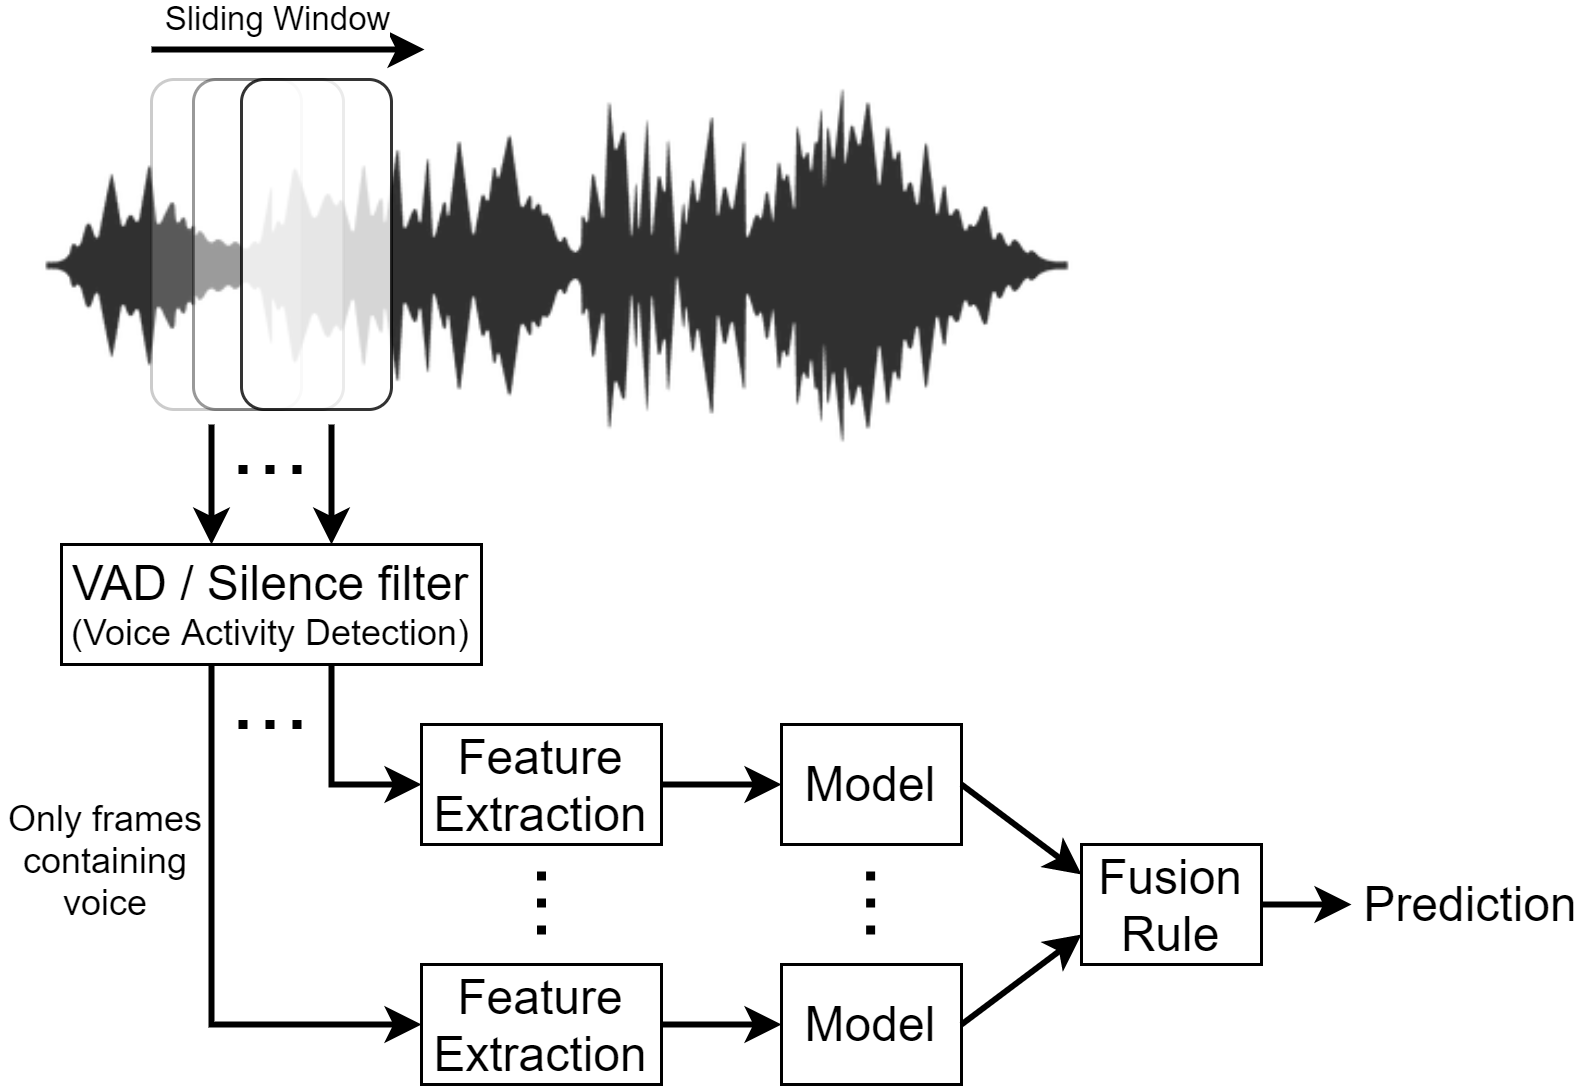
\includegraphics[scale=0.23]{End-To-End}
\caption{The end-to-end framework proposed consists of framing the input audio signal into several frames with appropriate overlapping percentage, a Voice Activity Detection module that filters out frames that do not contain voice, a feature extraction module, a neural network and a fusion rule.}
\end{figure*}

\section{Signals and Features}
As stated in Sec. I, we used the Google Speech Dataset V2. This dataset contains 105,829 audio files in .wav format (duration =  one second) divided in thirty classes, plus an additional class containing five different type of noise of variable duration (about ten seconds for each file).

The core words are "Yes", "No", "Up", "Down", "Left", "Right", "On", "Off", "Stop", "Go", "Zero", "One", "Two", "Three", "Four", "Five", "Six", "Seven", "Eight", and "Nine". To help distinguish unrecognized words, there are also ten auxiliary words that most speakers only say once: "Bed", "Bird", "Cat", "Dog", "Happy", "House", "Marvin", "Sheila", "Tree", and "Wow".

We decided to create two different datasets:
\begin{itemize}
\item the first one is made of ten classes ("Yes", "No", "Up", "Down", "Left", "Right", "On", "Off", "Stop", "Go"), where each class contains approximately 3,600 files;
\item the second is made of twenty-one classes ("Yes", "No", "Up", "Down", "Left", "Right", "On", "Off", "Stop", "Go", "Zero", "One", "Two", "Three", "Four", "Five", "Six", "Seven", "Eight", "Nine" and “Unknown”), where each class contains approximately 3,600 files, except for the “Unknown” class that contains all the remaining auxiliary words.
\end{itemize}

\subsection{Dataset Partitioning}
We divided both datasets into train-validation-test sets as suggested by Google Dataset’s README file and we used a split of 30K-3K-3K for the ten classes dataset and 84K-9K-11K for the twenty-one classes one. 

The training set is used to train the network, while the validation set is used to evaluate the network performance during the training and to allow early-stopping to save the model with the lowest validation error, preventing overfitting. The test set is used to evaluate the network’s final score that reaches the best performance.

\subsection{Features extraction}

We decided to study four different types of features in order to compare them and tried to see which was the best able to solve our problem:
\begin{itemize}
\item \textbf{No feature extraction}: we trained a specific model (1DCNN) directly on the raw signal (a 16,000 elements vector);
\item \textbf{80 Mels spectrogram}: we took the Fourier Transform of (a windowed excerpt of) the raw signal and mapped the powers of the spectrum obtained into the mel scale (using triangular overlapping windows);
\item \textbf{40 Mel-frequency cepstral\footnote{The cepstrum is the result of the Fourier Transform applied to the signal spectrum, in decibel.} coefficients (MFCC)}: the coefficients are obtained after the computation of the Discrete Cosine Transform (DCT) on the logarithm of the Mel spectrogram;
\item \textbf{40 MFCC + $\Delta$s}: matrix containing the MFCCs previously computed also considering their first and second derivatives.
\end{itemize}
We used the \textit{Librosa Python Library} to compute these features, in particular we used the following functions:
\begin{itemize}
\item \texttt{librosa.feature.melspectrogram(...)};
\item \texttt{librosa.power\_to\_db(...)};
\item \texttt{librosa.feature.mfcc(...)};
\item \texttt{librosa.feature.delta(...)}.
\end{itemize}

\section{Learning Framework}

\vspace{-1mm}
\subsection{1DCNN on raw data}
\begin{figure*}
\centering
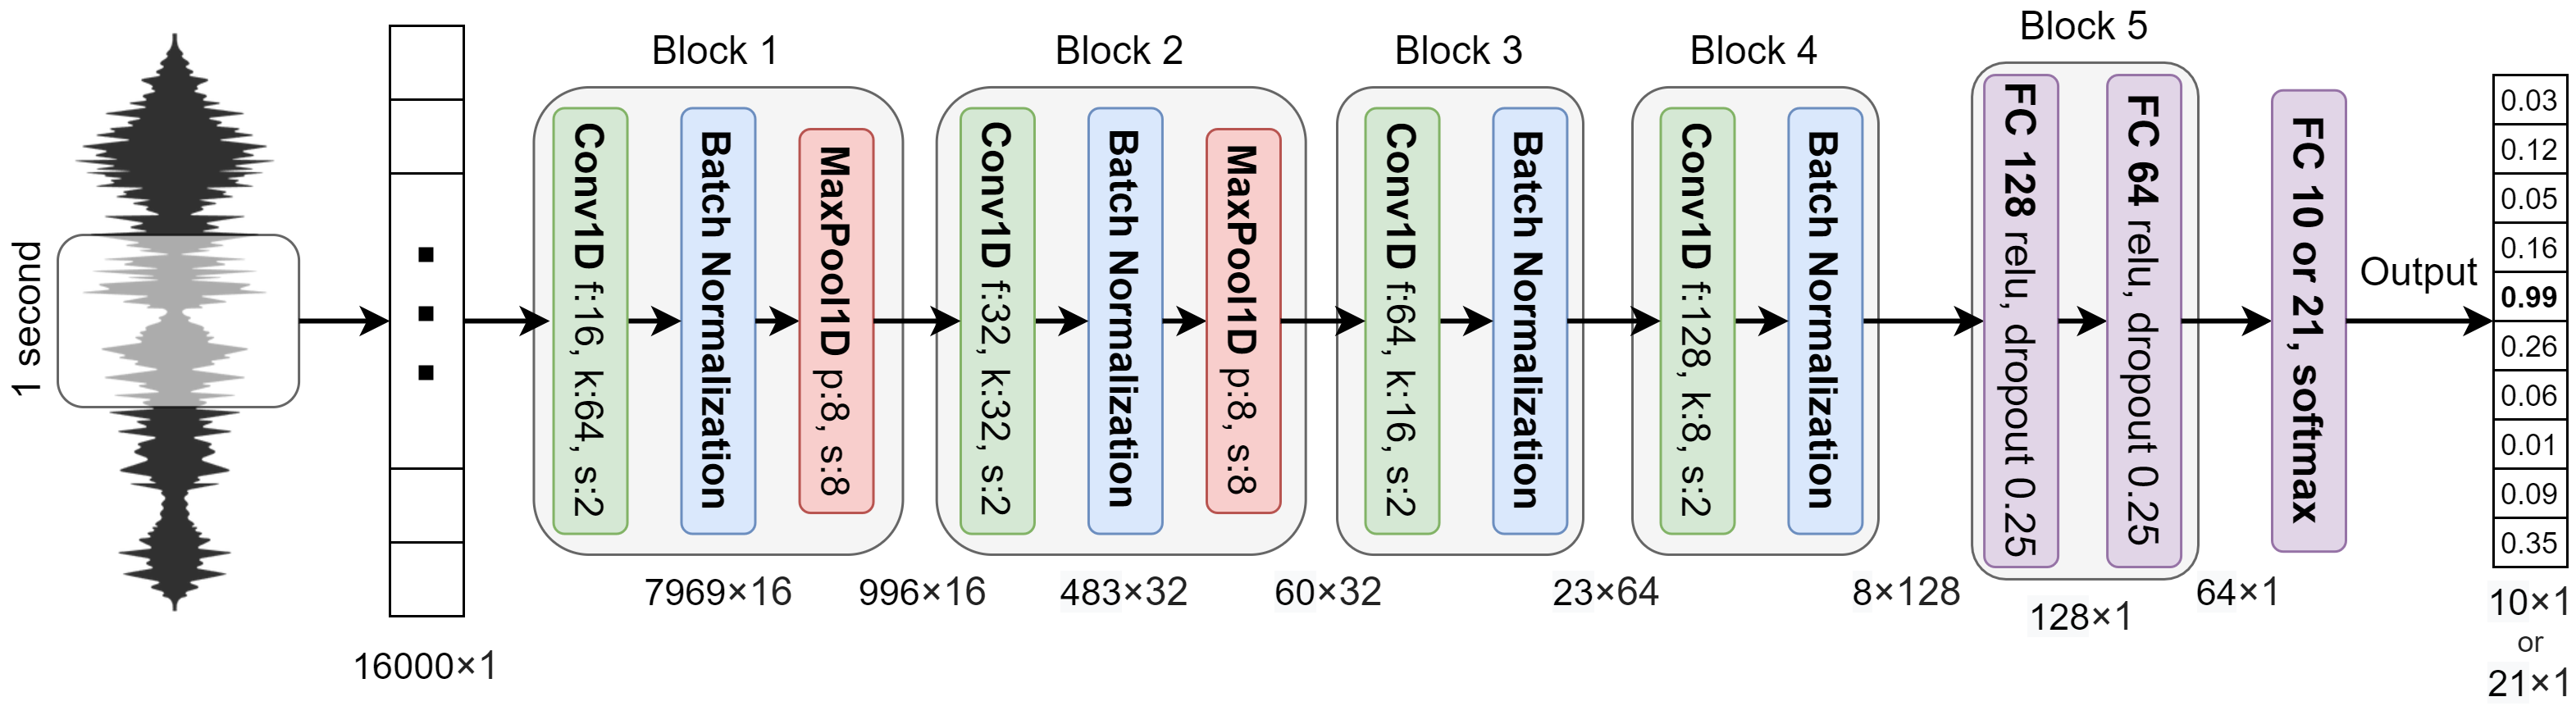
\includegraphics[scale=0.16]{1DCNN}
\caption{The architecture of the proposed 1D CNN model.}
\end{figure*}

The proposed architecture, shown in Fig. 2, is made of four convolutional layers interlaced with max pooling layers and followed by two fully connected layers and an output layer.

The input consists of an array of 16,000 dimensions, which represents a 1-second audio sample at 16kHz.
The proposed 1DCNN has large receptive fields in the first convolutional layers since it is assumed that the first layers should have a more “global view” of the audio signal. 

The output of the last pooling layer, for all feature maps, is flattened and represents the input for a fully connected layer. In order to reduce overfitting, batch normalization is applied after the activation function of each convolution layer. After the last pooling layer there are two fully connected layers with 128 and 64 neurons respectively; dropout is applied with a probability of 0.25 for both layers.

Keeping in mind the architecture shown in Fig. 2, it is possible to omit a signal processing module because the network is strong enough to extract relevant low and high-level information from the audio waveform.
In the case of multiclass classification, the number of neurons of the output layer is the number of classes. Using the \textit{softmax} as activation function for the output layer, each output neuron indicates the membership degree of the input samples for each class.

\subsection{DSConv Model}
This model uses Depthwise Separable Convolutions. A separable convolution uses less parameters, less memory and less computations than regular convolutional layers, and in general it even performs better.
There are two types of Separable Convolution: Spatial and Depthwise.

Spatial Separable Convolutions divide a kernel into two smaller kernels (e.g. division of a 3$\times$3 kernel into a 3$\times$1 and 1$\times$3 kernel). Instead of considering one convolution with 9 multiplications, we handled two convolutions with 3 multiplications each (6 in total) to achieve the same result. With a lower number of multiplications, the computational complexity significantly decreases, and the network is able to run and train faster.

Depthwise Separable Convolutions use kernels that cannot be split into two smaller kernels that apply two different convolutions: the \textit{depthwise convolution}, which result will be the input for the \textit{pointwise} (1$\times$1) one.

In Fig. 3 we show the difference between a normal 3D Convolution and a Depthwise one, and the final Depthwise Separable Convolutions block we used. 

In our work we adopted a Depthwise Separable CNN inspired by [3]. This CNN is made of a 2D CNNs followed by batch normalization and four or five DSConv2D layers. An average pooling, with padding 2$\times$2 and stride 2$\times$2, followed by a fully connected layer, is used in the end to provide global interaction and reduce the total number of parameters in the final layer.
We implemented three different variants: \textit{Large}, \textit{Medium} and \textit{Small}, described in the Tables at pages 5 and 6, where we tried to reduce the number of parameters still maintaining a good accuracy.

\begin{figure*}[t]
\centering
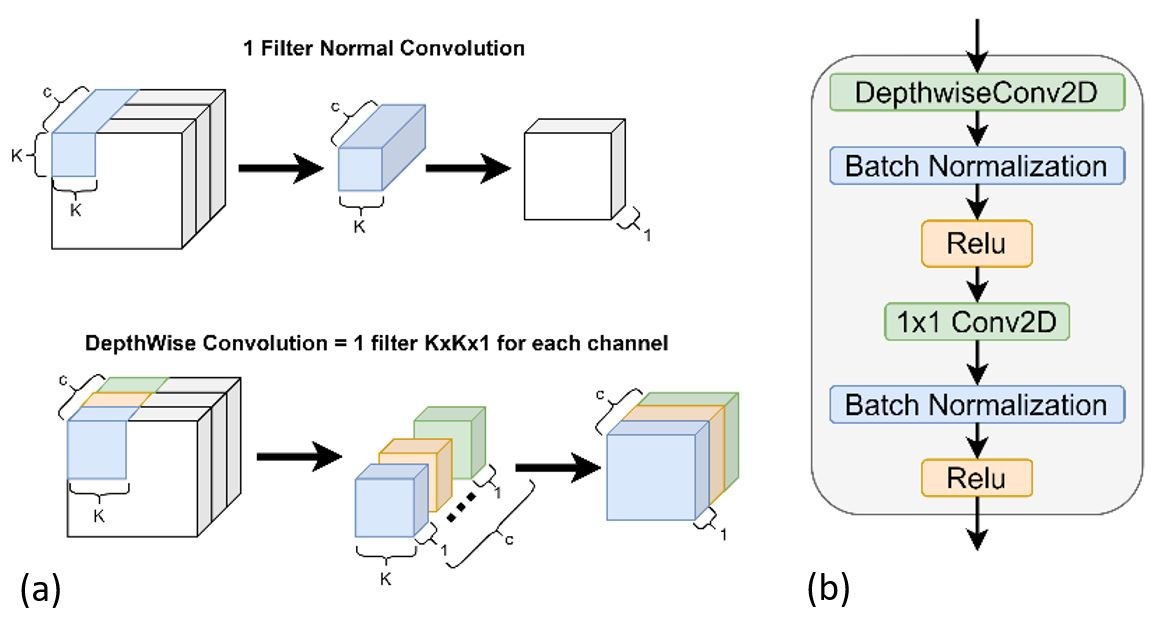
\includegraphics[scale=0.56]{confronto3}
\caption{Difference between normal convolution and depthwise convolution (left). DSConv layer (right).}
\end{figure*}
\begin{center}

\begin{table*}[]
\scalebox{1.28}{
\begin{tabular}{@{}llllllll@{}}
\toprule
\multicolumn{2}{c}{\multirow{2}{*}{\textbf{Model Size}}} &
  \multicolumn{6}{c}{\textbf{Layers}} \\ \cmidrule(l){3-8} 
\multicolumn{2}{c}{} &
  \textbf{Conv2D} &
  \textbf{DSConv2D 1} &
  \textbf{DSConv2D 2} &
  \textbf{DSConv2D 3} &
  \textbf{DSConv2D 4} &
  \textbf{DSConv2D 5} \\ \midrule
\textbf{Small} &
  \begin{tabular}[c]{@{}l@{}}\# Filters\\ Filter size\\ Stride\end{tabular} &
  \begin{tabular}[c]{@{}l@{}}64\\ 10$\times$4\\ 2$\times$2\end{tabular} &
  \begin{tabular}[c]{@{}l@{}}64\\ 3$\times$3\\ 1$\times$1\end{tabular} &
  \begin{tabular}[c]{@{}l@{}}64\\ 3$\times$3\\ 1$\times$1\end{tabular} &
  \begin{tabular}[c]{@{}l@{}}64\\ 3$\times$3\\ 1$\times$1\end{tabular} &
  \begin{tabular}[c]{@{}l@{}}64\\ 3$\times$3\\ 1$\times$1\end{tabular} &
  NA \\ \midrule
\textbf{Medium} &
  \begin{tabular}[c]{@{}l@{}}\#Filters\\ Filter size\\ Stride\end{tabular} &
  \begin{tabular}[c]{@{}l@{}}172\\ 10$\times$4\\ 1$\times$2\end{tabular} &
  \begin{tabular}[c]{@{}l@{}}172\\ 3$\times$3\\ 2$\times$2\end{tabular} &
  \begin{tabular}[c]{@{}l@{}}172\\ 3$\times$3\\ 1$\times$1\end{tabular} &
  \begin{tabular}[c]{@{}l@{}}172\\ 3$\times$3\\ 1$\times$1\end{tabular} &
  \begin{tabular}[c]{@{}l@{}}172\\ 3$\times$3\\ 1$\times$1\end{tabular} &
  NA \\ \midrule
\textbf{Large} &
  \begin{tabular}[c]{@{}l@{}}\# Filters\\ Filter size\\ Stride\end{tabular} &
  \begin{tabular}[c]{@{}l@{}}276\\ 10$\times$4\\ 1$\times$2\end{tabular} &
  \begin{tabular}[c]{@{}l@{}}276\\ 3$\times$3\\ 2$\times$2\end{tabular} &
  \begin{tabular}[c]{@{}l@{}}276\\ 3$\times$3\\ 1$\times$1\end{tabular} &
  \begin{tabular}[c]{@{}l@{}}276\\ 3$\times$3\\ 1$\times$1\end{tabular} &
  \begin{tabular}[c]{@{}l@{}}276\\ 3$\times$3\\ 1$\times$1\end{tabular} &
  \begin{tabular}[c]{@{}l@{}}276\\ 3$\times$3\\ 1$\times$1\end{tabular} \\ \bottomrule
\end{tabular}}
\caption{The configurations of the DSConv model layers considering different model sizes.}
\end{table*}
\end{center}

\subsection{Ensemble}
\vspace{-1mm}
As stated before, we built three kinds of ensembles (\textit{Large}, \textit{Medium} and \textit{Small}) in order to have models that can fit different hardware sizes.  The ensembles simply pick the two best models and compute the average of their final prediction, in this way we reached the best accuracy paying a high price: larger networks.

All models were trained with the \textbf{Google Tensorflow 2.1} Framework with \textbf{Keras} using the standard \textit{Sparse categorical cross entropy} and \textit{Nadam optimizer}. With a batch size of 32, the models were trained for 100 epochs with initial learning rate of $10^{-4}$. An early stopping with a patience of 10 epochs was applied to avoid overfitting.

\section{Results}
We trained each DSConv network for all the features we described in Section IV to see if there was any difference between each set. As stated before, we used two different datasets, one made of ten class and another one of twenty-one.

We found that the number of convolutional layers played a key role in detecting high-level concepts, both for the DSConv models and the 1DCNN one. The number of convolutional layers in our models was determined in an experiment using the audio files of the Google Speech Commands V2 Dataset.

We faced the overfitting problem, recognizing the importance of the early-stopping procedure during the training, comparing the test scores of the last epochs of the models with the best ones found by the \texttt{ModelCheckpoint} function of Keras (using the validation set).
It took some time, for us, to choose the best metrics to use to evaluate our models, and at the end we decided \textit{accuracy} was the best choice.

We also measured the prediction speed of each model with and without Feature Extraction. 
%We should not consider multiplication as metric because it is an indirect alternative for a direct metric such as latency.

Furthermore, we noticed that predicting one example or a batch made of ten examples required almost the same amount of time: this happened because TensorFlow makes tensors operations. In the final implementation this fact should be taken into account in order to minimize the computational cost.

In Tables II, III, IV, V and VI we summarized the accuracy and the speed prediction of our models: the 40 MFCCs + $\Delta$s one does not perform better, on the contrary the models have worse accuracy, a larger number of parameters and they are slower.
There is not so much difference between using 80 Mels or 40 MFCCs, calculating MFCC requires slightly more time since they are calculated after the Mels but MFCC requires almost half of the parameters.
The fastest network is the 1DCNN on raw data since it has not to calculate any feature extraction, but it is the worst in terms of accuracy.
The best accuracy is obtained by the ensemble network (the slower and larger model).
The smallest model is the DSConvSmall + 40 MFCCs with 127K parameters, 92.9\% accuracy and 38.23 ms of prediction speed.
\begin{center}
\begin{table}[]
\scalebox{1.38}{
\begin{tabular}{@{}cll@{}}
\cmidrule(l){2-3}
\multicolumn{1}{l}{} &
  \multicolumn{1}{c}{\textbf{\begin{tabular}[c]{@{}c@{}}10-commands\\ (30K-3K-3K)\end{tabular}}} &
  \multicolumn{1}{c}{\textbf{\begin{tabular}[c]{@{}c@{}}21-commands\\ (84K-9K-11K)\end{tabular}}} \\ \midrule
\textbf{Accuracy \%}   & 93.0   & 89.1   \\ \midrule
\textbf{\# parameters} & 257,018 & 257,733 \\ \midrule
\textbf{Speed (ms)}    & 28.71  & 28.25  \\ \bottomrule
\end{tabular}}
\begin{center}
\caption{1DCNN performances on 10 and 21-commands datasets.}
\end{center}
\end{table}
\end{center}

\begin{table*}[]
\scalebox{1.46}{
\begin{tabular}{@{}cllllll@{}}
\toprule
\multicolumn{1}{l}{\multirow{2}{*}{}} &
  \multicolumn{3}{c}{\textbf{\begin{tabular}[c]{@{}c@{}}10-commands\\ (30K-3K-3K)\end{tabular}}} &
  \multicolumn{3}{c}{\textbf{\begin{tabular}[c]{@{}c@{}}21-commands\\ (84K-9K-11K)\end{tabular}}} \\ \cmidrule(l){2-7} 
\multicolumn{1}{l}{}   & \textit{80 Mels} & \textit{40 MFCC} & \textit{40 + $\Delta$ MFCC} & \textit{80 Mels} & \textit{40 MFCC} & \textit{40 + $\Delta$ MFCC} \\ \midrule
\textbf{Accuracy \%}   & \textbf{96.0}               & 95.3             & 93.9                     & 93.4             & \textbf{93.7}              & 92.7                      \\ \midrule
\textbf{\# parameters} & 874,930           & \textbf{571,330}           & 1,178,530                  & 1,375,881          & \textbf{738,321}              & 2,013,441                      \\ \midrule
\textbf{\begin{tabular}[c]{@{}c@{}}Speed (ms)\\ Speed with FE\end{tabular}} &
  \begin{tabular}[c]{@{}l@{}}\textbf{33.39}\\ \textbf{41.44}\end{tabular} &
  \begin{tabular}[c]{@{}l@{}}30.24\\ 45.32\end{tabular} &
  \begin{tabular}[c]{@{}l@{}}33.42\\ 44.25\end{tabular} &
  \begin{tabular}[c]{@{}l@{}}33.79\\ 41.62\end{tabular} &
  \begin{tabular}[c]{@{}l@{}}\textbf{30.87}\\ \textbf{39.66}\end{tabular} &
  \begin{tabular}[c]{@{}l@{}}33.13\\ 44.62\end{tabular} \\ \bottomrule
\end{tabular}}
\caption{DSConv Large performances on 10 and 21-commands datasets.}
\end{table*}

\begin{table*}[]
\scalebox{1.48}{
\begin{tabular}{@{}cllllll@{}}
\toprule
\multicolumn{1}{l}{\multirow{2}{*}{}} &
  \multicolumn{3}{c}{\textbf{\begin{tabular}[c]{@{}c@{}}10-commands\\ (30K-3K-3K)\end{tabular}}} &
  \multicolumn{3}{c}{\textbf{\begin{tabular}[c]{@{}c@{}}21-commands\\ (84K-9K-11K)\end{tabular}}} \\ \cmidrule(l){2-7} 
\multicolumn{1}{l}{}   & \textit{80 Mels} & \textbf{\textit{40 MFCC}} & \textit{40 + $\Delta$ MFCC} & \textit{80 Mels} & \textit{40 MFCC} & \textit{40 + $\Delta$ MFCC} \\ \midrule
\textbf{Accuracy \%}   & 94.3             & \textbf{95.0}               & 94.8                     & \textbf{92.7}             & 92.2             & 91.7                      \\ \midrule
\textbf{\# parameters} & 469,398           & \textbf{262,998}           & 675,798                   & 832,673           & \textbf{399,233}           & 1,266,113                      \\ \midrule
\textbf{\begin{tabular}[c]{@{}c@{}}Speed (ms)\\ Speed with FE\end{tabular}} &
  \begin{tabular}[c]{@{}l@{}}30.75\\ 38.49\end{tabular} &
  \begin{tabular}[c]{@{}l@{}}\textbf{29.55}\\ \textbf{38.23}\end{tabular} &
  \begin{tabular}[c]{@{}l@{}}30.76\\ 41.82\end{tabular} &
  \begin{tabular}[c]{@{}l@{}}\textbf{32.25}\\ \textbf{39.72}\end{tabular} &
  \begin{tabular}[c]{@{}l@{}}30.01\\ 46.76\end{tabular} &
  \begin{tabular}[c]{@{}l@{}}33.03\\ 47.08\end{tabular} \\ \bottomrule
\end{tabular}}
\caption{DSConv Medium performances on 10 and 21-commands datasets.}
\end{table*}

\begin{table*}[]
\scalebox{1.48}{
\begin{tabular}{@{}cllllll@{}}
\toprule
\multicolumn{1}{l}{\multirow{2}{*}{}} &
  \multicolumn{3}{c}{\textbf{\begin{tabular}[c]{@{}c@{}}10-commands\\ (30K-3K-3K)\end{tabular}}} &
  \multicolumn{3}{c}{\textbf{\begin{tabular}[c]{@{}c@{}}21-commands\\ (84K-9K-11K)\end{tabular}}} \\ \cmidrule(l){2-7} 
\multicolumn{1}{l}{}   & \textit{80 Mels} & \textbf{\textit{40 MFCC}} & \textit{40 + $\Delta$ MFCC} & \textit{80 Mels} & \textit{40 MFCC} & \textit{40 + $\Delta$ MFCC} \\ \midrule
\textbf{Accuracy \%}   & 92.5             & \textbf{92.9}             & 92.5                      & \textbf{90.0}               & 89.2             & 86.5                      \\ \midrule
\textbf{\# parameters} & 300,618           & \textbf{127,818}           & 473,418                      & 604,757           & \textbf{241,877}           & 967,637                      \\ \midrule
\textbf{\begin{tabular}[c]{@{}c@{}}Speed (ms)\\ Speed with FE\end{tabular}} &
  \begin{tabular}[c]{@{}l@{}}31.00\\ 38.31\end{tabular} &
  \begin{tabular}[c]{@{}l@{}}\textbf{29.27}\\ \textbf{38.23}\end{tabular} &
  \begin{tabular}[c]{@{}l@{}}30.54\\ 40.23\end{tabular} &
  \begin{tabular}[c]{@{}l@{}}\textbf{32.86}\\ \textbf{37.97}\end{tabular} &
  \begin{tabular}[c]{@{}l@{}}29.48\\ 48.15\end{tabular} &
  \begin{tabular}[c]{@{}l@{}}30.31\\ 40.99\end{tabular} \\ \bottomrule
\end{tabular}}
\caption{DSConv Small performances on 10 and 21-commands datasets.}
\end{table*}

\begin{table*}[]
\scalebox{0.91}{
\begin{tabular}{@{}cllllll@{}}
\toprule
\multicolumn{1}{l}{\multirow{2}{*}{}} &
  \multicolumn{3}{c}{\textbf{\begin{tabular}[c]{@{}c@{}}10-commands\\ (30K-3K-3K)\end{tabular}}} &
  \multicolumn{3}{c}{\textbf{\begin{tabular}[c]{@{}c@{}}21-commands\\ (84K-9K-11K)\end{tabular}}} \\ \cmidrule(l){2-7} 
\multicolumn{1}{l}{} &
  \multicolumn{1}{c}{\textit{\begin{tabular}[c]{@{}c@{}}\textbf{Large}\\ DSConv L 80 Mels\\ +\\ DSConv L 40 MFCC\\ +\\ DSConv L 40 MFCC $\Delta$\end{tabular}}} &
  \multicolumn{1}{c}{\textit{\begin{tabular}[c]{@{}c@{}}\textbf{Medium}\\DSConv L 40 MFCC\\ +\\ DSConv M 80 Mels\\ +\\ DSConv M 40 MFCC\end{tabular}}} &
  \multicolumn{1}{c}{\textit{\begin{tabular}[c]{@{}c@{}}\textbf{Small}\\DSConv M 40 MFCC\\ +\\ DSConv M 80 Mels\\ +\\ DSConv S 40 MFCC\end{tabular}}} &
  \multicolumn{1}{c}{\textit{\begin{tabular}[c]{@{}c@{}}\textbf{Large}\\DSConv L 80 Mels\\ +\\ DSConv L 40 MFCC\\ +\\ DSConv L 40 MFCC $\Delta$\end{tabular}}} &
  \multicolumn{1}{c}{\textit{\begin{tabular}[c]{@{}c@{}}\textbf{Medium}\\DSConv L 40 MFCC\\ +\\ DSConv M 80 Mels\\ +\\ DSConv L 40 MFCC\end{tabular}}} &
  \multicolumn{1}{c}{\textit{\begin{tabular}[c]{@{}c@{}}\textbf{Small}\\DSConv L 40 MFCC\\ +\\ DSConv M 80 Mels\\ +\\ DSConv L 40 MFCC\end{tabular}}} \\ \midrule
\textbf{Accuracy \%}   & 96.8    & 96.4   & 95.6 & 95.2     & 95.0   & 94.2 \\ \midrule
\textbf{\# parameters} & 2,624,790 & 1,303,726 & 691,463 & 2,498,019 & 1,970,227 & 1,379,431 \\ \midrule
\textbf{Speed (ms)}     & 131.01   & 122.04    & 106.09 & 125.9    & 114.21    & 109.03 \\ \bottomrule
\end{tabular}}
\caption{Ensemble performances on 10 and 21-commands datasets.}
\end{table*}

%\pagebreak
\section{Concluding Remarks}
In this paper, an end-to-end architecture for the Keyword Spotting Task has been proposed. We built two neural networks and an ensemble between the best models.

The 1DCNN consists of five convolutional layers. Instead of using handcrafted static filterbanks (such as the ones used to extract MFCC features), the proposed 1DCNN learns the filters directly from the audio waveform. The other network receives as input features 80Mels, 40MFCCs or 40MFCCs + $\Delta$s and consists of four or five DSConv layers. Furthermore, the 1DCNN is faster than the other models, but unfortunately it does not reach the same accuracy.

As we can see from the results, all the features work well but 40MFCCs seems slightly better that the others, the 1DCNN on raw waveform performed the worst way.
We then reduced the number of parameters of the DSConv model by lowering the filters number for each convolution. We proposed three version of the DSConv model: \textit{Large}, \textit{Medium} and \textit{Small}.

Our models achieve excellent results but we did not beat the state of the art accuracy of 97.4\% reached in [4]. In TABLE VII at page 7 there is a summary of our model compared with the state of the art.
We noticed that if we picked more frames per second, as described in the end-to-end architecture, the model had many “points of view” of the word, so in the real world it could actually perform better than the test accuracy measured. In various tests we made, the networks (even the 1DCNN, the one with the worst accuracy) captured all the words we were saying thank to the multiple windows – fusion rule technique.

Further improvements could be explored with the SincConv, Attention Mechanism and LSTMs.

The code can be found on the following GitHub page: \texttt{https://github.com/ivaste/KeyWordSpotting}.

\begin{figure*}
\centering
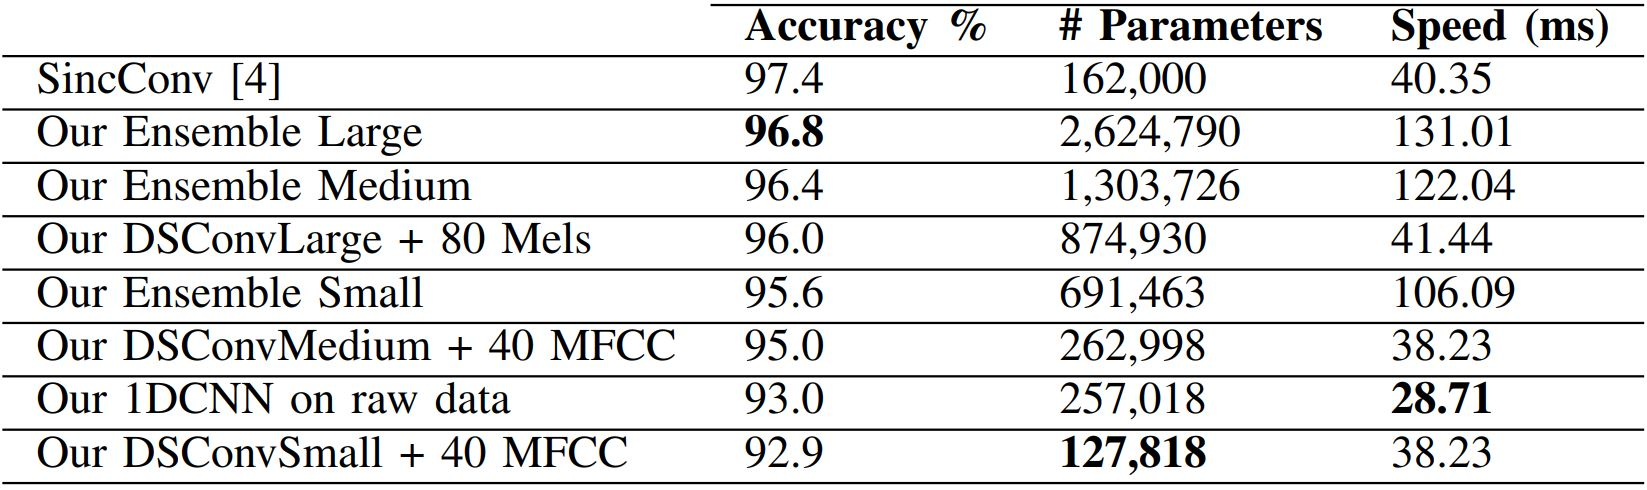
\includegraphics[scale=0.3]{tab1}
\begin{center}
TABLE VII: The architecture of the proposed 1D CNN model.
\end{center}
\end{figure*}

\begin{figure*}
\centering
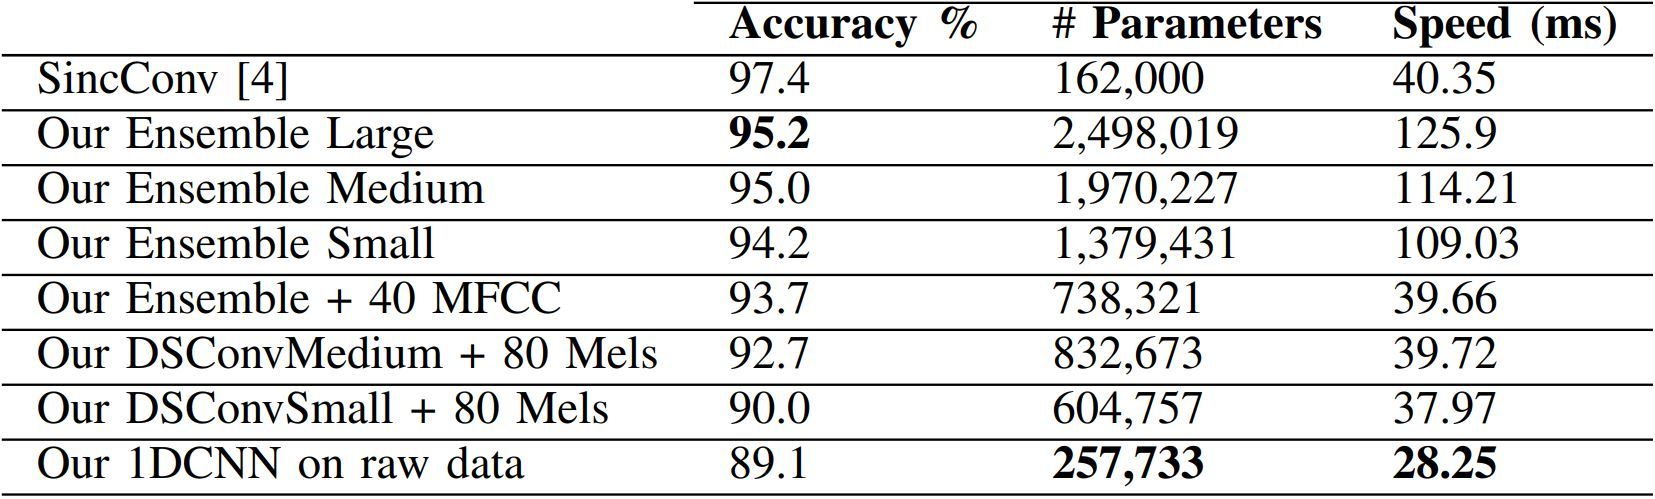
\includegraphics[scale=0.3]{tab2}
\begin{center}
TABLE VIII: Summary of the 21-commands networks performances.
\end{center}
\end{figure*}

\newpage
\section*{Work Setup}
The decided to organize our work in the following way:
\begin{itemize}
\item \textbf{Literature research:}: Stefano Ivancich and Luca Masiero;
\item \textbf{Dataset preparation}: Stefano Ivancich;
\item \textbf{1DCNN}: Luca Masiero;
\item \textbf{DSConv}: Stefano Ivancich;
\item \textbf{Ensemble}: Stefano Ivancich;
\item \textbf{Feature Extraction methods}: Luca Masiero;
\item \textbf{Full Demo}: Stefano Ivancich;
\item \textbf{\LaTeX\xspace document}: Luca Masiero and Stafano Ivancich;
\end{itemize}

\section*{What we have learnt as students}
We cannot say we faced an easy problem. We learnt how to research and select papers from scientific literature, set-up a machine learning project, design an end-to-end architecture for Speech Recognition, debug and improve a machine learning model and write with \LaTeX\xspace a scientific paper.

We had several problems using our university cluster, even if it is new and powerful hundreds of students and researchers enqueue jobs everyday, our laptops resulted ten times faster (the vast majority of the tests run on an ASUS ROG GL703GM \textit{Scar Edition}, with processor Intel Core i7-8750H Hexa-Core, Nvidia  GeForce GTX 1060 and 16GB RAM memory).

\begin{thebibliography}{1}
\bibitem{1}
L. R. Rabiner, “A tutorial on hidden markov models and selected applications in speech recognition,” Proceedings of the IEEE, vol. 77, pp. 257–286, Feb 1989.

\bibitem{2}
Sajjad Abdoli, Patrick Cardinal and Alessandro Lameiras Koerich. \textit{End-to-End Environmental Sound Classification using a 1D Convolutional Neural Network}. arXiv:1904.08990v1 [cs.SD] 18 Apr 2019

\bibitem{3}
Yundong Zhang, Naveen Suda, Liangzhen Lai and Vikas Chandra. \textit{Hello Edge: Keyword Spotting on Microcontrollers}. arXiv:1711.07128v3 [cs.SD] 14 Feb 2018.

\bibitem{4}
Simon Mittermaier, Ludwig Kurzinger, Bernd Waschneck and Gerhard Rigoll. \textit{Small-Footprint Keyword Spotting on Raw Audio Data with Sinc-Convolutions}. arXiv:1911.02086v1 [eess.AS] 5 Nov 2019

\bibitem{5}
G Alon. \textit{Key-word spotting—the base technology for speech analytics}. Natural Speech Communications, 2005 - crmxchange.com
\end{thebibliography}
\end{document}

%\begin{table*}[]
%\scalebox{1.75}{
%\begin{tabular}{llll}
%\cline{2-4}
%                           & \textbf{Accuracy \%} & \textbf{\# Parameters} & \textbf{Speed (ms)} \\ %\hline
%SincConv [4]                   & 97.4                 & 162,000                & 40.35               \\ %\hline
%Our Ensemble Large         & \textbf{96.8}        & 2,624,790              & 131.01              \\ %\hline
%Our Ensemble Medium        & 96.4                 & 1,303,726              & 122.04              \\ %\hline
%Our DSConvLarge + 80 Mels  & 96.0                 & 874,930                & 41.44               \\ %\hline
%Our Ensemble Small         & 95.6                 & 691,463                & 106.09              \\ %\hline
%Our DSConvMedium + 40 MFCC & 95.0                 & 262,998                & 38.23               \\ %\hline
%Our 1DCNN on raw data         & 93.0                 & 257,018                & \textbf{28.71}      \\ %\hline
%Our DSConvSmall + 40 MFCC   & 92.9                 & \textbf{127,818}       & 38.23               \\ %\hline
%\end{tabular}}
%\caption{Summary of the 10-commands networks performances.}
%\end{table*}
%
%\begin{table*}[]
%\scalebox{1.8}{
%\begin{tabular}{llll}
%\cline{2-4}
%                          & \textbf{Accuracy \%}   & \# \textbf{Parameters}    & \textbf{Speed (ms)}     %\\ \hline
%SincConv [4]                  & 97.4          & 162,000          & 40.35          \\ \hline
%Our Ensemble Large        & \textbf{95.2} & 2,498,019        & 125.9          \\ \hline
%Our Ensemble Medium       & 95.0          & 1,970,227        & 114.21         \\ \hline
%Our Ensemble Small        & 94.2          & 1,379,431        & 109.03         \\ \hline
%Our Ensemble + 40 MFCC     & 93.7          & 738,321          & 39.66          \\ \hline
%Our DSConvMedium + 80 Mels & 92.7          & 832,673          & 39.72          \\ \hline
%Our DSConvSmall + 80 Mels  & 90.0          & 604,757          & 37.97          \\ \hline
%Our 1DCNN on raw data         & 89.1          & \textbf{257,733} & \textbf{28.25} \\ \hline
%\end{tabular}}\\
%\caption{Summary of the 21-commands networks performances.}
%\end{table*}
